\documentclass[10pt,a4paper]{article}
\usepackage[utf8]{inputenc}
\usepackage[danish]{babel}
\usepackage[T1]{fontenc}
\usepackage[margin=2cm]{geometry}
\usepackage{array}
\usepackage{ragged2e}
\usepackage{fancyhdr}
\usepackage{graphicx}
\usepackage{lastpage}
\usepackage{hyperref}
\hypersetup{
    colorlinks=true,       % Brug farvet tekst i stedet for rammer
    linkcolor=black,       % Intern link farve (f.eks. indholdsfortegnelse)
    citecolor=black,
    urlcolor=black,        % Farve på URL'er (sort = ingen synlig farve)
    pdfborder={0 0 0},     % Fjern rammer helt (vigtigst for sidetal og links)
}
\usepackage{url}
\def\UrlBreaks{\do\/\do-\do_}
\usepackage{makecell}
\usepackage{xcolor}
\usepackage{titling}
\usepackage{booktabs}

% Kolonnetype
\newcolumntype{P}[1]{>{\RaggedRight\hangindent=1em\arraybackslash}p{#1}}

% --- Header og footer ---
\pagestyle{fancy}
\fancyhf{}   % Ryd alt først

% Footer (uændret)
\fancyfoot[L]{%
  \raisebox{-0.4\height}{%
    
\includegraphics[width=2.5cm]{Billeder/Logo/OesterbroJagttegn_clean.png}%
  }%
}
\fancyfoot[R]{Side \thepage\ af \pageref{LastPage}}

% ← HER TILFØJES DATOEN I HEADEREN
\fancyhead[R]{\footnotesize \today}
\fancyhead[L]{\footnotesize Hold: Østerbro Jagttegn Vinter Flex 3}

% Eventuelt en tynd linje under header (valgfri – fjern hvis du ikke vil have den)
\renewcommand{\headrulewidth}{0.2pt}
\renewcommand{\footrulewidth}{0pt}

\begin{document}

% Starter direkte med indhold
\centering

\subsection*{Praktisk info}
\vspace{0.2cm}

\begin{flushleft}

\textbf{Jagttegnskursus}

\vspace{0.3cm}

Kære kommende jagttegnsaspirant

\vspace{0.2cm}

Tak fordi du har valgt at tage undervisningen hos Østerbro Jagttegn. Her følger praktisk information om kurset. Kurset sammenkøres med et andet hold fra 2. modul. 

\vspace{0.4cm}
\textbf{Formalia}

\vspace{0.1cm}
Når jagttegnskursus påbegyndes skal aspiranten generere et Jæger ID:\\
\url{https://sgavmst.dk/natur-og-jagt/jagttegn/jagttegnsaspirant}

\vspace{0.2cm}
Jæger ID sendes til Aleksander, som verificerer tilmeldingen hos Styrelsen:\\
\url{https://forms.gle/bb8U1L8rG7F3RM449}

\vspace{0.4cm}
\textbf{Lokation}

\vspace{0.1cm}
Den teoretiske del af undervisningen afholdes på Østerbro:

\vspace{0.1cm}
\hspace{1em} Soldalen 8, 2100 Kbh Ø\\
\hspace{1em} \url{https://maps.app.goo.gl/ZoqJgyLXoeqLDwNcA}

\begin{center}
    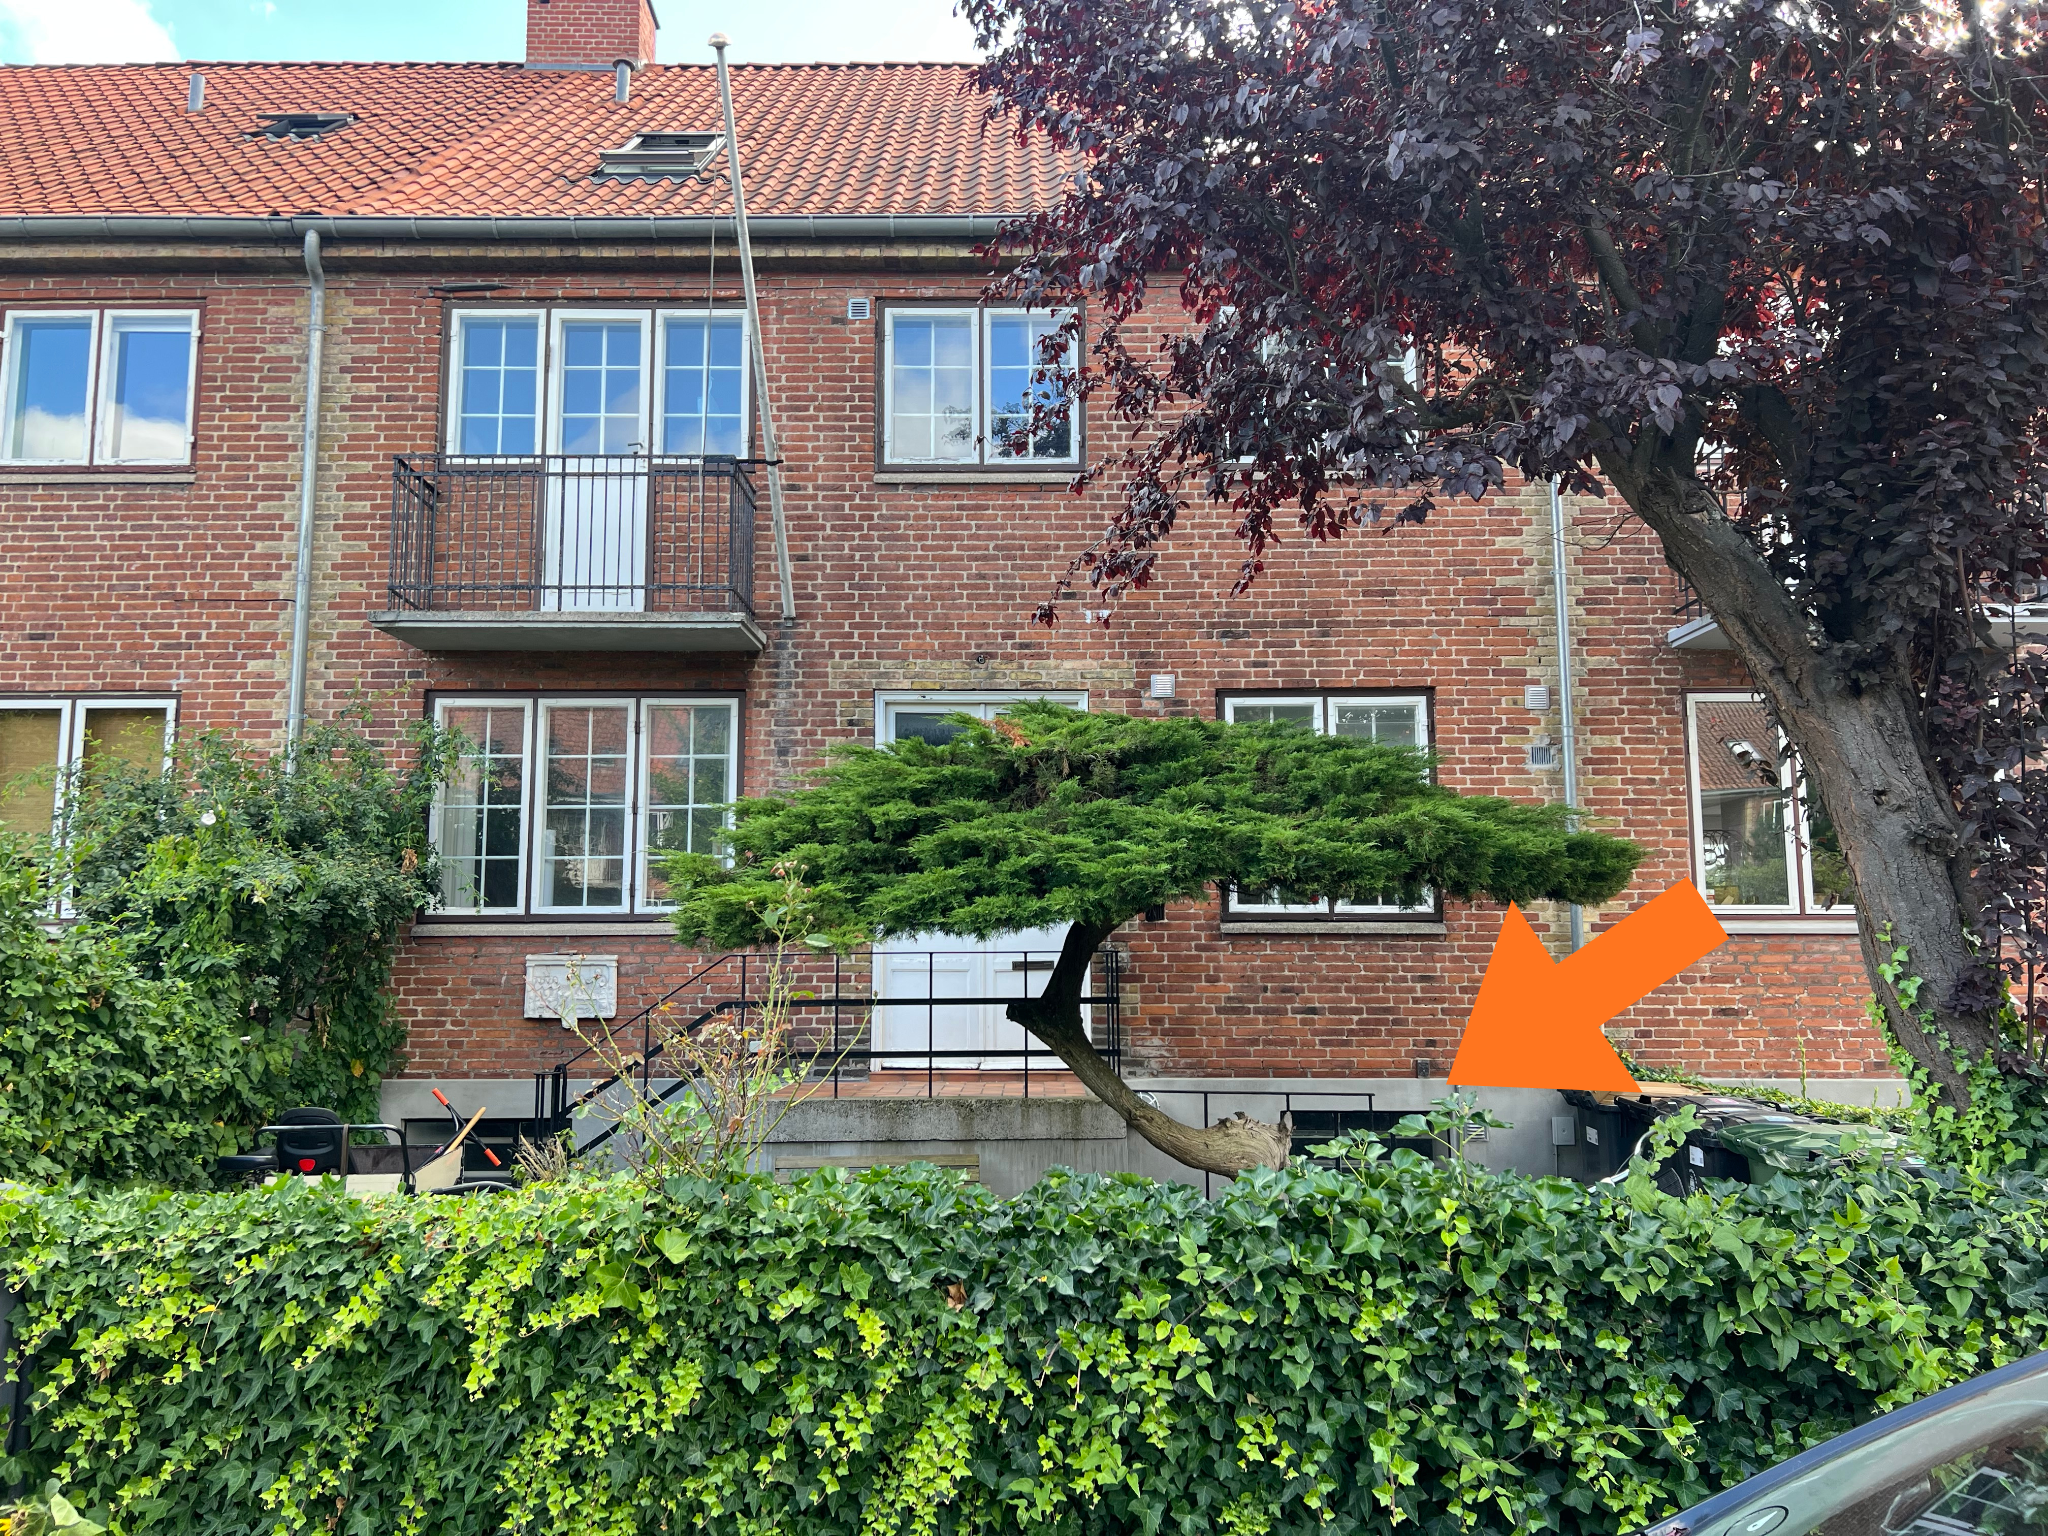
\includegraphics[width=0.4\textwidth]{Billeder/Andet/Indgang.png}
\end{center}

\vspace{0.2cm}
Gå ind via kælderdøren til højre for hovedindgangen. Der er tre timers gratis parkering i området, så husk at sætte p-skiven. Svanemøllen Station ligger tre minutter til fods fra adressen. Kommer du på cykel, kan den parkeres i forhaven.

\vspace{0.2cm}
Den praktiske del af undervisningen (afstandsbedømmelse og skydning) afvikles på forsvarets øvelsesterræn i Birkerød og supplerende afstandsbedømmelse i Mindelunden på Østerbro:

\vspace{0.1cm}
\hspace{1em} Hørsholm og Omegns Jagtforening Flugtskydebanen, 3460 Birkerød\\
\hspace{1em} \url{https://maps.app.goo.gl/9HGMBBcETuUc4Tyj6}
\\
\vspace{0.2cm}
\hspace{1em} Mindelunden, Major Anders Lassens Vej, 2100 Kbh Ø\\
\hspace{1em} \url{https://maps.app.goo.gl/frJmr4sNSVdjDe6h8}

\vspace{0.4cm}
\textbf{Kursusmateriale}

\vspace{0.1cm}
Teoriprøven, som udgør den ene halvdel af jagtprøven, består af 40 multiple choice spørgsmål i forskellige variationer. Teorispørgsmål kan trænes via portalen \url{https://osjagttegn.dk}.

\vspace{0.2cm}
Undervisningen tager udgangspunkt i lovtekster, bekendtgørelser mm.\ (se lektionsplan herunder). Der findes flere lærebogssystemer, som alle kan anvendes i forbindelse med kurset, men dette er ikke et krav. Man kan fint nøjes med lovtekster og præsentationer.

\vspace{0.2cm}
Det komplette pensum til jagtprøven er angivet i bilagslisten nedenfor med aktive links. Hvor der er angivet §, kapitel etc. er det kun de specifikke punkter, der udgør pensum. 

\vspace{0.4cm}
\textbf{Kommunikation}

\vspace{0.1cm}
Løbende kommunikation igennem kurset køres via WhatsApp i gruppen \emph{Østerbro Jagttegn vf2\_26}:\\
\url{https://chat.whatsapp.com/BMfd13gMv2RL8rK3jt25jy}

\vspace{0.2cm}
Præsentationer, bekendtgørelser mm.\ deles via Google Drive:\\
\url{https://drive.google.com/drive/folders/1iLtHqLLlpJ-f5kI5OEOSgUxoz1dal9t4?usp=sharing}

\vspace{0.4cm}
\textbf{Forløb}

\vspace{0.1cm}
Herunder overblik over undervisningen. Bemærk at der er mødepligt til alle de 8 teoretiske og praktiske lektioner.

\vspace{0.3cm}


\vspace{0.4cm}
Jeg glæder mig til at gøre jer klar til jagtprøven. Skriv eller ring endelig, hvis der er spørgsmål. Denne tekst ligger også som PDF i Google Drive.

\vspace{0.3cm}
Mange hilsner

\vspace{0.2cm}
Aleksander Sønder\\
Tlf. 26 16 06 30

\end{flushleft}

\vspace{0.4cm}

\subsection*{Lektionsplan}
\vspace{0.2cm}

\begin{tabular}{|P{4.5cm}|P{1.5cm}|P{5cm}|P{5.5cm}|}
\hline
\textbf{Dato} & \textbf{Lektion} & \textbf{Emner} & \textbf{Materiale} \\
\hline


% LEKTION 1

\makecell[l]{Onsdag 18/11 \\ (Svanemøllen) \\ 19:50–22:05} &
Lektion 1 &
\makecell[l]{%
Introduktion \\ 
Jagtprøven \\
Våbenhåndtering \\
Jagttider \\
Skadevoldende vildt \\
Artsbestemmelse \\
Vildtbiologi \\
Svømmeænder%
} &
\makecell[l]{%
Bogen Jagttegn: s. 9-10, 11-24 \\ 188, \\ 190-192. 59-72 \\
\\
Bilag 1 \\
Bilag 2 (ikke bilagene) \\
Bilag 3 (§ 51 og 52) \\
Bilag 4 (§§ 39-45) \\
Bilag 9  \\
Bilag 12 (§§ 1-5, bilag 1)\\
%
} \\
\hline

% LEKTION 2

\makecell[l]{Torsdag 19/11 \\ (Svanemøllen) \\ 19:50–22:05} &
Lektion 2 &
\makecell[l]{%
Artsfredning \\
Dykænder, Gravænder,\\
Skalleslugere \\  
Våbenbekendtgørelse \& cirkulære \\
Årefodede, Storkefugle, Gæs, \\
Repetition Teori 1 \\
Våbenhåndtering \\ 
Jagt fra kunstige skjul \\ 
Rovfugle \\ 
Jægerudtryk 1. del%
} &
\makecell[l]{%
Bogen Jagttegn: s. 72-85, 57-59, \\ 86-89, 41-56, 368, 127-137 \\
\\
Bilag 5 (§ 5 stk. 1, § 6, 11, \\ §§ 20-21, 24-25, § 49, 52)  \\
Bilag 7 (§ 16) \\
Bilag 10 (Kapitel 1)\\
Bilag 11 (§§ 1-9, § 10 stk. 1, § 11, \\ §§ 25-31)\\
Bilag 2 (bilag 2)
%
} \\
\hline

% LEKTION 3
\makecell[l]{Torsdag 10/12 \\ (Mindelunden \& Svanemøllen) \\ 19:50–22:05} &
Lektion 3 &
\makecell[l]{%
Afstandsbedømmelse \\
Vadefugle, Fasanfugle \\
Vildtforvaltning \\
Repetition Teori 1-2 \\
Udsætning af vildt \\
Æggebekendtgørelsen \\
Måger, Vandhøns, \\ 
Spurvefugle, Duer \\
Jægerudtryk 2. del
%
} &
\makecell[l]{%
Bogen Jagttegn: s. 96-115, 183-198, \\ 116-126, 90-95 \\ 
\\
Bilag 4 (§§ 37-45) \\
Bilag 10 (Kapitel 6-7)\\
Bilag 8 (§§ 1-2, § 14) 
%
} \\
\hline

% LEKTION 4
\makecell[l]{Torsdag 14/1 \\ (Svanemøllen) \\ 19:50–22:05} &
Lektion 4 &
\makecell[l]{%
Hovdyr \\
De jagtetiske regler \\
Rovdyr \\
Naturbeskyttelse \\
Natura 2000 \\
Våbenhåndtering \\
Repetition Teori 1-3 \\
Gnavere, støttetandede \\
De jagtetiske regler for kronvildt\\
Våbenkendskab \\
Jægerudtryk 3. del%
} &
\makecell[l]{%
Bogen Jagttegn: s. 138–181, 199-241 \\ 
\\
Bilag 13 \\
Bilag 14 \\
Bilag 16 (§ 3, §§ 38-39)
Bilag 17%
} \\
\hline

% LEKTION 5
\makecell[l]{Torsdag 11/2 \\ (Svanemøllen) \\ 19:50–22:05} &
Lektion 5 &
\makecell[l]{%
Ammunition \\
Jagtudøvelse \\
Jagtformer \\
Jagthunde \\
Våbenhåndtering \\
Repetition Lektion 1-4 \\
Håndtering af nedlagt vildt \\
Skudafgivelse \\
Eftersøgning af vildt% 
} &
\makecell[l]{%
Bogen Jagttegn: s. 315-417 \\
\\
Bilag 15 (Kapitel 49, s. 96-100) \\
Bilag 19 (§§ 1-6)%
} \\
\hline

% LEKTION 6
\makecell[l]{Torsdag 11/3 \\ (Svanemøllen) \\ 19:50–22:05} &
Lektion 6 &
\makecell[l]{%
Opsamling \\
Våbenhåndtering \\
} &
\makecell[l]{% 
} \\
\hline

% LEKTION 7-8
\makecell[l]{Torsdage (fleksibelt) \\ (Hørsholm) \\ 9:00–15:00 (45 min)} &
Lektion 7-8 &
\makecell[l]{%
Afstandsbedømmelse \\
Våbenhåndtering \\
Skydning \\
} &
\makecell[l]{% 
} \\
\hline
\end{tabular}

\vspace{1cm}

\subsection*{Bilagsliste}
\begin{frame}{}
{\footnotesize
\setlength{\tabcolsep}{3pt}
\renewcommand{\arraystretch}{1.25}

\centering
\begin{tabular}{|P{1.1cm}|P{5.2cm}|P{3.2cm}|P{6.0cm}|}
\hline
\textbf{Bilag} & \textbf{Navn} & \textbf{Paragraffer (Pensum)} & \textbf{Link} \\
\hline

1 & Instruks for jagtprøven & & \url{https://sgavmst.dk/media/2w5hrceb/2025_instruks-for-jagtproeven.pdf} \\
\hline

2 & Retningslinjer for spørgsmål der stilles i den skriftlige del af jagtprøven (inkl. Jægerudtryk) & & \url{https://sgavmst.dk/media/vkffhaxl/2025_retningslinjer-for-hvilke-spoergsmaal-der-stilles-i-den-skriftlige-jagtproeve.pdf} \\
\hline

3 & \textbf{Jagttegnsbekendtgørelsen} Bekendtgørelse om jagttegn (BEK nr 238 af 27/02/2025) & § 51, § 52 & \url{https://www.retsinformation.dk/eli/lta/2025/238} \\
\hline

4 & \textbf{Jagt- og vildtforvaltningsloven} Bekendtgørelse af lov om jagt og vildtforvaltning (LBK nr 639 af 26/05/2023) & §§ 1-34, §§ 37–45 & \url{https://www.retsinformation.dk/eli/lta/2023/639} \\
\hline

5 & Bekendtgørelse om våben og ammunition m.v. (BEK nr 2531 af 20/12/2021) & § 5 stk. 1, § 6, § 11, §§ 20–21, §§ 24–25, § 49, § 52 & \url{https://www.retsinformation.dk/eli/lta/2021/2531} \\
\hline

6 & Bekendtgørelse om våben og ammunition der må anvendes til jagt mv. (BEK nr 1479 af 05/12/2023) & §§ 1–3 & \url{https://www.retsinformation.dk/eli/lta/2023/1479} \\
\hline

7 & Cirkulære om våben og ammunition m.v. (CIR1H nr 10066 af 29/10/2025) & § 16 & \url{https://www.retsinformation.dk/eli/retsinfo/2025/10066} \\
\hline

8 & Bekendtgørelse om æg fra vilde fugle og registrering af ægsamlinger (BEK nr 936 af 27/06/2016) & §§ 1–2, § 14 & \url{https://www.retsinformation.dk/eli/lta/2016/936} \\
\hline

9 & \textbf{Vildtskadebekendtgørelsen} Bekendtgørelse om vildtskader (BEK nr 708 af 27/08/2026) & Hele bekendtgørelsen & \url{https://www.retsinformation.dk/eli/lta/2026/708} \\
\hline

10 & Bekendtgørelse om udsætning af vildt, jagtmåder og jagtredskaber (BEK nr 1652 af 19/12/2017) & §§ 1–14 & \url{https://www.retsinformation.dk/eli/lta/2017/1652} \\
\hline

11 & \textbf{Artsfredningsbekendtgørelsen} Bekendtgørelse om fredning af visse dyre- og plantearter og pleje af tilskadekommet vildt (BEK nr 521 af 25/03/2021) & §§ 1-9, § 10, stk. 1, og § 11, §§ 25-31 & \url{https://www.retsinformation.dk/eli/lta/2021/521} \\
\hline

12 & \textbf{Jagttidsbekendtgørelsen} Bekendtgørelse om jagttid for visse pattedyr og fugle m.v. (BEK nr 470 af 17/05/2024) & §§ 1-5, De generelle jagttider nævnt i bilag 1 & \url{https://www.retsinformation.dk/eli/lta/2024/470} \\
\hline

13 & De jagtetiske regler & Hele dokumentet & \url{https://sgavmst.dk/natur-og-jagt/om-at-gaa-paa-jagt/jagtetiske-regler} \\
\hline

14 & De jagtetiske regler for kronvildt & Hele dokumentet & \url{https://naturstyrelsen.dk/media/ku0mld41/de-jagtetiske-regler-for-kronvildt.pdf} \\
\hline

15 & Hygiejnevejledningen (vejledning nr. 10099 af 20. december 2023) & Kapitel 49 (s. 96–100) & \url{https://foedevarestyrelsen.dk/Media/639141887265760386/Vejledning%20om%20f%C3%B8devarehygiejne_nr_9700_af_24_07_2025.pdf} \\
\hline

16 & \textbf{Naturbeskyttelsesloven} Bekendtgørelse af lov om naturbeskyttelse (LBK nr 927 af 28/06/2024) & § 3, §§ 37–38 & \url{https://www.retsinformation.dk/eli/lta/2024/927} \\
\hline

17 & Natura 2000 områderne & & \url{https://sgavmst.dk/natur-og-jagt/naturindsatser/natura-2000} \\
\hline

18 & \textbf{Våbenloven} Bekendtgørelse af lov om våben og eksplosivstoffer m.v. (LBK nr 1736 af 26/08/2021) & §§ 2 a og 2 b, §§ 6 b og 6 d & \url{https://www.retsinformation.dk/eli/lta/2021/1736} \\
\hline

19 & Bekendtgørelse om eftersøgning og aflivning af nødstedt vildt (BEK nr 827 af 24/06/2016) & §§ 1–6 & \url{https://www.retsinformation.dk/eli/lta/2016/827} \\
\hline

\end{tabular}
}
\end{frame}

\vspace{1cm}


\end{document}